\documentclass[a4paper,11pt]{article}
\usepackage{graphicx}
\usepackage[bottom]{footmisc}
 
\begin{document}
\title{Considering Computational Intelligence}
\author{Jessica E. Snyder}
\date{\today}
\maketitle

\begin{abstract}
The objective of this exercise is to learn about computation design. For an hour a day for 100 days, the author plans to research and document this subject. If after 100 days the author has nothing to add to this topic, that is interesting. Else: the author will have a stockpile of new thoughts and understanding for the next 100 days.

Many things seem impossible, but are really just uncomfortable. 

\end{abstract}

Keywords: Computational intelligence, computational design, generative alghorithm

\tableofcontents

\section{Let's begin}
Computational processes extend the patterns human see across larger and larger sets of numeric values. What if humans could ask the computational processes for help finding the patterns, instead of giving instructions? Maybe we already have. 
 
\section{How do computers design?}

Generative designs modeled refugee camps in Luxeumborg \cite{daher2017data}:

\begin{enumerate}

\item City officials seek to forecast future needs for events with none or limited local precedent, refugee camps for example, by using computational models based on data. 

\item A technological asset in resource allocation is computational design. 
\item Context-aware adaptation and usage requirements can e assigned to urban fragments. 
\item The policy makers of cities seek development policites that balance situational, technical, and human factors with flexibility to accomodate future needs. 
\item Specifically, cities to shelter people in camps. 
\item Human migration is increasing due to climate change and human activities. 
\item Many levels of districts, cities, and territories would benefit from resilience. 
\item Luxembourg stood up a public program to develop three container villages for refugees. 
\item The computational tool is for policy makers and humanitarians to design the spatial character of refugee camps. 
\item The model optizes for space layout. 
\item Policy makers can choose between several scenarios during planning. 
\item During early planning, a computaitonal tool can keep solutions bounded to finite resources and needs. 
\item This data-based approach facilitates collaboration between different disciplines and stake holders.  


\end{enumerate}

\section{How do bees make decisions?}


Let's learn from foraging bees: \cite{dunlap2016foraging}
\begin{enumerate}
\item Social and personal information guide foraging bumble bees. 
\item Bees trust social information over personal, if the social information is reliable. 
\item Bees learn and assign credibility to both personal and social information.
\item Bees recorgnize fellow bees - conspecific individuals. 
\item Bees priortize the actions of conspecific individuals over other behavior. 
\item Bees make decisions. 
\item Bees consier social and pesonal information (assigning both types different weights) during decision making. 
\item Bees assign the reliability of information. 
\item Bees compare new information to something of relevance in the environment to determine consistency and theefore reliability. 
\item The bee determine reliability and the modulates communication signals and determines which stimuli to continue payng attention to. 
\item Bumble bes (Bombus impatiens) decide which flower to approach based personal and social information. Personal information includes past experience that certain color flowers have a reward. Social information includes waching other bees choose flowers. 
\item Bees prefer social information to personal if there is any reward, instead of their own experience. 
\item If social information is completely unreliable, then bees rely on their own personal information - flower color.  
\item Bee foraging behaves like other bees when it is similar to their expectations. If other bees are behaving outside of expectations, bees will rely on their own experience. 
\end{enumerate}




The natural order has evolved solutions decision making skills - like way-finding for flying insects. Understanding the balancing act between numerous data streams (i.e. threat level from predators, environmental hazards, maintaining a mental map of the area, acheiving a goal, finding food) provides a starting point to program robotic swarms for cooperation. 

"Computational intelligence techniques have widespread applications in the field of engineering process optimization, which typically comprises of multiple conflicting objectives. An efficient hybrid algorithm for solving multi‐objective optimization, based on particle swarm optimization (PSO) and artificial bee colony optimization (ABCO) has been proposed in this paper. The novelty of this algorithm lies in allocating random initial solutions to the scout bees in the ABCO phase which are subsequently optimized in the PSO phase with respect to the velocity vector. The last phase involves loyalty decision‐making for the uncommitted bees based on the waggle dance phase of ABCO. This procedure continues for multiple generations yielding optimum results. The algorithm is applied to a real life problem of intercity route optimization comprising of conflicting objectives like minimization of travel cost, maximization of the number of tourist spots visited and minimization of the deviation from desired tour duration. Solutions have been obtained using both pareto optimality and the classical weighted sum technique. The proposed algorithm, when compared analytically and graphically with the existing ABCO algorithm, has displayed consistently better performance for fitness values as well as for standard benchmark functions and performance metrics for convergence and coverage."\cite{beed2020hybrid}


\section{Optimizing design}

The most efficient way to dope a hollow fiber with engineered diatoms is to use additive manufacturing \cite{dalwadi2015understanding}.

Efficiency to close the loop on life support systems. Efficiency means as close to a closed loop system as possible - converting the carbon dioxide produced by the 4-person crew, into bicarbonate fed to a microbial farm, that is fed to the crew as a protein source, who in turn produce carbon dioxide. 
Additive manufacturing for reliability: Additive manufacturing is uniquely equipped for remote operation because individual processes (dispensing, motion along a tool path, integrated movements) can be integrated into a programmable build cycle. Because of automation comes with process control, the results are reproducible. Reproducibility means the results is reliable and with an iterative design process, the optimal set of parameters will produce a desired result.  

A reliable biofunctional filter is possible now as never before due to recent advancements in additive biomanufacturing. The project team includes the inventors of a pioneering technology well suited for this multi-material application, which has been developed for tissue engineering and translated into this biological industrial design project. The new process integrates several material delivery systems in a single computer aided design and manufacturing environment. By having thermal extrusion, pneumatic extrusion, and electrospinning in a single device, the proposal team can custom build a hollow fiber made of hydrogel and polymer. The process deposits load-bearing and biofunctional materials side-by-side during a layer-by-layer manufacturing process. The team will investigate the hypothetical benefit of automating the manufacturing process as compared to an off-the-shelf solution where the diatoms must be introduced to the hollow fiber matrix after construction using a series of injections, which is not automated or well controlled. 

3D printing made unidirectional graded filters possible as never before and improved filtration efficiency [Dalwadi, 2015]. A gradient of pores (compared to a uniform network) maximizes absorption (or reactions between effluent and matrix in general) and minimizes potential blockages. The computational and fabrication tools used for filters can be translated from filters to remove toxins to a hollow fiber to convert carbon dioxide to bicarbonate. In addition to engineered biological function and optimized material formulation, gradient structures can improve the system performance in a way that is well controlled and impossible using off-the-shelf solutions.

To achieve the objective, we build on the outcomes of earlier tasks that engineer the diatom to convert carbon dioxide to bicarbonate, identify the optimal hydrogel (likely a blend of poly (aspartic acid) / poly(vinyl alcohol) ) and geometric properties of the filter (i.e. height, diameter, wall thickness).
The technical plan is an iterative cycle of three task: (1) computational model,  (2) rapid prototyping, and (3) performance test. The computational model takes the system inputs (rate of carbon dioxide entering the system, conversion per diatom, geometric properties of the filter) and desired performance (percentage of carbon converted, system cost, energy usage). The rapid prototyping is building the hollow fiber embedded with diatoms. The performance test measures the percentage carbon converted and energy used to inform the next iteration of design and for comparison to off-the-shelf solutions. 

\section{Creating Information}


To protect patient privacy, imaginary human genomic records were made using machine learning and random noise. This high quality synthetic data provides medical researchers a resource for computational studies \cite{yelmen2021creating}.

\section{Technical plan}

Open SCAD is a programmable modeling software. The model was made from design parameters on the struct width and spacing. These geometric variables could be connected to physical parameters to make the model a solution based on data and performance for other problems. 

Open SCAD is free and open source software \footnote{
OpenSCAD: The Programmers Solid 3D CAD Modeller https://www.openscad.org/}.

\begin{figure}
  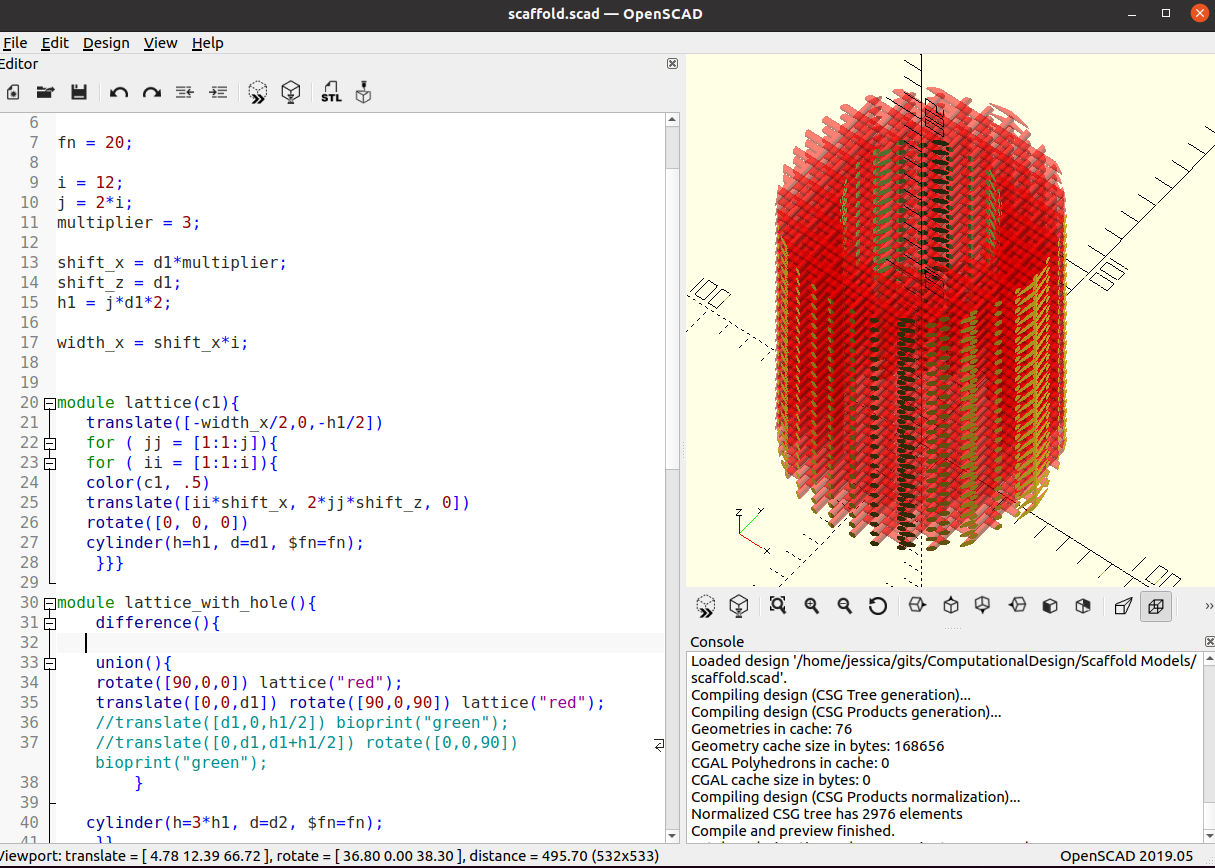
\includegraphics[width=\linewidth]{day05.png}
  \caption{Model of a hybrid scaffold.}
  \label{fig:boat1}
\end{figure}

\section{Counterculture ideas}

The Agori, a class of Hindu Fakir, violate all rules of the caste system because they have no class prejudice and believe God made all is sacred, so no act of man can mak something unsacred \cite{balfour1897life}. They do not distinguish between the living and the dead or food and waste. All are welcome to join. The only criteria is all members must be a disciple of a guru for at least 6 months before admission. The practice of eating and drinking from a human skull is thought to be rooted in self-abasement. One of the three Agori sects, the Ghure sect is the most extreme, eating anything, the only exception being horse. Hindus view the Aghori wth veneration. 


\bibliographystyle{acm}
\bibliography{references}

\newpage

\end{document}